%/*% pdflatex -file-line-error -interaction nonstopmode %

\documentclass{article}
\usepackage{graphicx}
\graphicspath{ {./images/} }
\usepackage{amsmath}
\usepackage{amsfonts}
\usepackage{bookmark}
\usepackage{exercises}
\usepackage{amsthm}
\usepackage{yhmath}
\newcommand*{\oldneg}{\mathord{\sim}}

\theoremstyle{definition}
\newtheorem{definition}{Definition}

\setlength{\parindent}{.5in}
\setlength{\parskip}{12pt}

\title{1.8 Exercises}
\begin{document}
\maketitle

\section*{1}
You can use the discrimant of a quadratic equation ot determine the equation's number and type of solutions.

\section*{2}
I could not solve this, mainly due to the fact that I did not know what $v_0$ was.


\section*{3}
$x^2-4x-5=0\newline\rightarrow x=\frac{4\pm \sqrt{(-4)^2-4(1)(-5)}}{2(1)}\newline\rightarrow \frac{4+6}{2}\vee \frac{4-6}{2}\newline\rightarrow 
x=5\vee x=-1$

\section*{4}
$x^2-6x+7=0\newline\rightarrow x=\frac{6\pm \sqrt{(-6)^2-4(1)(7)}}{2(1)}\newline\rightarrow \frac{6+2\sqrt{2}}{2}\vee \frac{6-2\sqrt{2}}{2}\newline
\rightarrow x=3+\sqrt{2}\vee x=3-\sqrt{2}$

\section*{5}
$t^2+8t+19=0\newline\rightarrow x=\frac{-8\pm \sqrt{(8)^2-4(1)(19)}}{2(1)}\newline\rightarrow \frac{-8\pm 2i\sqrt{3}}{2}\newline\rightarrow 
x=-4+i\sqrt{3}\vee x=-4-i\sqrt{3}$

\section*{6}
$x^2-16x+7=0\newline\rightarrow x=\frac{16\pm\sqrt{(-16)^2-4(1)(7)}}{2(1)}\newline\rightarrow \frac{16\pm \sqrt{228}}{2(1)}\newline\rightarrow 
x=8+2\sqrt{57}\vee x=8-2\sqrt{57}$

\section*{7}
$8w^2-8w+2=0\newline\rightarrow x=\frac{8\pm\sqrt{(-8)^2-4(8)(2)}}{2(8)}\newline\rightarrow \frac{8\pm 0}{16}\newline\rightarrow x=\frac{1}{2}$

\section*{8}
$5p^2-10p=0\newline\rightarrow x=\frac{10\pm\sqrt{(-10)^2-4(5)(0)}}{2(5)}\newline\rightarrow \frac{10\pm 10}{20}\newline\rightarrow x=0\vee x=2$

\section*{9}
$4x^2-8x+1=0\newline\rightarrow x=\frac{8\pm\sqrt{(-8)^2-4(4)(1)}}{2(4)}\newline\rightarrow \frac{8\pm \sqrt{48}}{8}\newline\rightarrow 
x=\frac{2+\sqrt{3}}{2}\vee x=\frac{2-\sqrt{3}}{2}$

\section*{10}
$6u^2+4u+11=0\newline\rightarrow x=\frac{-4\pm\sqrt{(4)^2-4(6)(11)}}{2(6)}\newline\rightarrow \frac{-4\pm\sqrt{-248}}{12}\newline\rightarrow 
x=\frac{-2+i\sqrt{62}}{6}\vee x=\frac{-2-i\sqrt{62}}{6}$

\section*{11}
$3r^2-8r-9=0\newline\rightarrow x=\frac{8\pm\sqrt{(-8)^2-4(3)(-9)}}{2(3)}\newline\rightarrow \frac{8\pm \sqrt{172}}{6}\newline\rightarrow 
x=\frac{4+\sqrt{43}}{3}\vee x=\frac{4-\sqrt{43}}{3}$

\section*{12}
$2x^2-16x+50=0\newline\rightarrow x=\frac{16\pm\sqrt{(-16)^2-4(2)(50)}}{2(2)}\newline\rightarrow \frac{16\pm\sqrt{-144}}{4}\newline\rightarrow 
x=4+3i\vee x=4-3i$, and thus, the correct answer is A.

\section*{13}
$3w^2-12w=-12\newline\rightarrow 3w^2-12w+12=0\newline\rightarrow w=\frac{12\pm\sqrt{(-12)^2-4(3)(12)}}{2(3)}\newline\rightarrow \frac{12\pm 0}{6}
\newline\rightarrow w=2$

\section*{14}
$x^2+6x=-15\newline\rightarrow x^2+6x+15=0\newline\rightarrow x=\frac{-6\pm\sqrt{(6)^2-4(1)(15)}}{2(1)}\newline\rightarrow \frac{-6\pm \sqrt{-24}}{2}
\newline\rightarrow x=-3+i\sqrt{6}\vee x=-3-i\sqrt{6}$

\section*{15}
$s^2=-14-3s\newline\rightarrow s^2+3s+14=0\newline\rightarrow s=\frac{-3\pm\sqrt{(3)^2-4(1)(14)}}{2(1)}\newline\rightarrow \frac{-3\pm\sqrt{-47}}{2}\newline
\rightarrow s=-\frac{3}{2}+\frac{\sqrt{47}}{2}i \vee s=-\frac{3}{2}-\frac{\sqrt{47}}{2}i$

\section*{16}
$-3y^2=6y-10\newline\rightarrow -3y^2-6y+10=0\newline\rightarrow y=\frac{6\pm\sqrt{(-6)^2-4(-3)(10)}}{2(-3)}\newline\rightarrow \frac{6\pm\sqrt{156}}{-6}
\newline\rightarrow y=\frac{-2-\sqrt{39}}{3}\vee y=\frac{-2+\sqrt{39}}{3}$

\section*{17}
$3-8v-5v^2=2v\newline\rightarrow -5v^2-10v+3=0\newline\rightarrow v=\frac{10\pm\sqrt{(-10)^2-4(-5)(3)}}{2(-5)}\newline\rightarrow 
v=\frac{5+2\sqrt{10}}{-5}\vee v=\frac{5-2\sqrt{10}}{-5}$

\section*{18}
$7x-5+12x^2=-3x\newline\rightarrow 12x^2+10x-5=0\newline\rightarrow x=\frac{-10\pm\sqrt{10^2-4(12)(-5)}}{2(12)}\newline\rightarrow 
x=\frac{-5+\sqrt{85}}{12}\vee x=\frac{-5-\sqrt{85}}{12}$

\section*{19}
$4x^2+3=x^2-7x\newline\rightarrow 3x^2+7x+3=0\newline\rightarrow x=\frac{-7\pm\sqrt{7^2-4(3)(3)}}{2(3)}\newline\rightarrow 
x=\frac{-7+\sqrt{13}}{6}\vee x=\frac{-7-\sqrt{13}}{6}$

\section*{20}
$6-2t^2=9t+15\newline\rightarrow -2t^2-9t-9=0\newline\rightarrow t=\frac{9\pm\sqrt{(-9)^2-4(-2)(-9)}}{2(-2)}\newline\rightarrow 
t=6\vee t=3$

\section*{21}
$4+9n-3n^2=2-n\newline\rightarrow -3n^2+10n+2=0\newline\rightarrow n=\frac{-10\pm\sqrt{10^2-4(-3)(2)}}{2(-3)}\newline\rightarrow 
n=\frac{-5+\sqrt{31}}{-3}\vee n=\frac{-5-\sqrt{31}}{-3}$

\section*{22}
Quadratic Formula:\newline
$z^2+15z+24=-32\newline\rightarrow z^2+15z+56=0\newline\rightarrow z=\frac{-15\pm\sqrt{15^2-4(1)(56)}}{2(1)}\newline\rightarrow 
z=-8\vee z=-7$\newline 
Factoring:\newline $(z+8)(z+7)=0\newline\rightarrow z=-8\vee z=-7$

\section*{23}
Quadratic Formula:\newline $x^2-5x+10=4\newline\rightarrow x^2-5x+6=0\newline\rightarrow x=\frac{5\pm\sqrt{(-5)^2-4(1)(6)}}{2(1)}\newline\rightarrow 
x=3\vee x=2$\newline
Factoring:\newline $x^2-5x+6=0\newline\rightarrow (x-3)(x-2)=0\newline\rightarrow x=3\vee x=2$

\section*{24}
Quadratic Formula:\newline $m^2+5m-99=3m\newline\rightarrow m^2+2m-99=0\newline\rightarrow m=\frac{-2\pm\sqrt{(2)^2-4(1)(-99)}}{2(1)}\newline\rightarrow 
m=-11\vee x=9$\newline
Factoring:\newline $m^2+2m-99=0\newline\rightarrow (m+11)(m-9)=0\newline\rightarrow m=-11\vee m-9$ 

\section*{25}
Quadratic Formula:\newline
$s^2-s-3=s\newline\rightarrow s^2-2s-3=0\newline\rightarrow s=\frac{2\pm\sqrt{(-2)^2-4(1)(-3)}}{2(1)}\newline\rightarrow s=3\vee -1$\newline
Factoring:\newline $s^2-2s-3=0\newline\rightarrow (s-3)(s+1)=0\newline\rightarrow s=3\vee s=-1$

\section*{26}
Quadratic Formula:\newline 
$r^2-4r+8=5r\newline\rightarrow r^2-9r+8=0\newline\rightarrow r=\frac{9\pm\sqrt{(-9)^2-4(1)(8)}}{2(1)}\newline\rightarrow r=8\vee r=1$\newline
Factoring:\newline $r^2-9r+8=0\newline\rightarrow (r-8)(r-1)\newline\rightarrow r=8\vee r=1$

\section*{27}
Quadratic Formula:\newline
$3x^2+7x-24=13x\newline\rightarrow 3x^2-6x-24=0\newline\rightarrow r=\frac{6\pm\sqrt{(-6)^2-4(3)(-24)}}{2(3)}\newline\rightarrow r=4\vee r=-2$\newline 
Factoring:\newline $3x^2-6x-24=0\newline\rightarrow (3x-12)(x+2)=0\newline\rightarrow x=4\vee x=-2$

\section*{28}
Quadratic Formula:\newline
$45x^2+57x+1=5\newline\rightarrow 45x^2+57x-4=0\newline\rightarrow x=\frac{-57\pm\sqrt{(57)^2-4(45)(-4)}}{2(45)}\newline\rightarrow x=\frac{6}{90}=\frac{1}
{15}
\vee x=-\frac{4}{3}$\newline 
Factoring:\newline $45x^2+57x-4=0\newline\rightarrow (15x-1)(3x+4)=0\newline\rightarrow x=\frac{1}{15}\vee x=-\frac{4}{3}$

\section*{29}
Quadratic Formula:\newline 
$5p^2+40p+100=25\newline\rightarrow 5p^2+40p+75=0\newline\rightarrow p=\frac{-40\pm\sqrt{40^2-4(5)(75)}}{2(5)}\newline\rightarrow p=-5\vee p=-3$\newline 
Factoring:\newline
$5p^2+40p+75=0\newline\rightarrow (5p+15)(p+5)=0\newline\rightarrow p=-3\vee p=-5$

\section*{30}
$9n^2-42n-162=21n\newline\rightarrow 9n^2-63n-162=0\newline\rightarrow n=\frac{63\pm\sqrt{(-63)^2-4(9)(-162)}}{2(9)}\newline\rightarrow n=-2\vee n=9$
\newline Factoring:\newline $9n^2-63n-162=0\newline\rightarrow (9n-81)(n+2)=0\newline\rightarrow n=9\vee n=-2$

\section*{31}
Discriminant: $(-8)^2-4(1)(16)=0=0$ and thus, this has one real solution.

\section*{32}
Discriminant: $7^2-4(1)(11)=5>0$ and thus, this has two real solutions.

\section*{33}
Discriminant: $8^2-4(8)(3)=-32<0$ and thus, this has two imaginary solutions.

\section*{34}
Discriminant: $1^2-4(-4)(-14)=-223<0$ and thus, this has two imaginary solutions. 

\section*{35}
Discriminant: $20^2-4(5)(21)=-20<0$ and thus, this has two imaginary solutions.

\section*{36}
Equation: $8z-10=z^2-7z+3\newline\rightarrow -z^2+15z-13=0$\newline Discriminant: $15^2-4(-1)(-13)=173>0$ and thus, this has two real solutions.

\section*{37}
Equation: $8n^2-4n+2=5n-11\newline\rightarrow 8n^2-9n+13=0$\newline Discriminant: $(-9)^2-4(8)(13)=-335<0$ and thus, this has two imaginary solutions.

\section*{38}
Equation: $5x^2+16x=11x-3x^2\newline\rightarrow 8x^2+5x=0$\newline Discriminant: $5^2-4(8)(0)=25>0$ and thus, this has two real solutions.

\section*{39}
Equation: $7r^2-5=2r+9r^2\newline\rightarrow -2r^2-2r-5=0$\newline Discriminat: $(-2)^2-4(-2)(-5)=-36<0$ and thus, this has two imaginary solutions.

\section*{40}
Equation: $16t^2-7t=17t-9\newline\rightarrow 16t^2-24t+9=0$. Solve by Factoring:\newline $(4t)^2-24t+3^2=0\newline\rightarrow (4t-3)^2=0\newline\rightarrow 
t=\frac{3}{4}$

\section*{41}
Equation: $7x-3x^2=85+2x^2+2x\newline\rightarrow -5x^2+5x-85=0\newline\rightarrow -5(x^2-x+17)=0\newline\rightarrow x^2-x+17=0$ Solve by 
completing the square:\newline $x^2-x=-17\newline\rightarrow x^2-x+\frac{1}{4}=-\frac{67}{4}\newline\rightarrow (x-\frac{1}{2})^2=-\frac{67}{4}\newline
\rightarrow x-\frac{1}{2}=\pm\sqrt{-\frac{67}{4}}\newline\rightarrow x=\frac{1}{2}\pm i\frac{\sqrt{67}}{2}$

\section*{42}
Equation: $4(x-1)^2=6x+2\newline\rightarrow 4(x^2-2x+1)=6x+2\newline\rightarrow 4x^2-8x+4=6x+2\newline\rightarrow 4x^2-14x+2=0\newline\rightarrow 
2(2x^2-7x+1)=0\newline\rightarrow 2x^2-7x+1=0\newline\rightarrow$ Solve by using the quadratic formula:\newline $x=\frac{7\pm\sqrt{(-7)^2-4(2)(1)}}{2(2)}
\newline\rightarrow x=\frac{7\pm\sqrt{41}}{4}\newline\rightarrow x=\frac{7+\sqrt{41}}{4}\vee x=\frac{7-\sqrt{41}}{4}$

\section*{43}
Equation: $25-16v^2=12v(v+5)\newline\rightarrow 25-16v^2=12v^2+60v\newline\rightarrow -28v^2-60v+25=0\newline\rightarrow$ Solve by factoring:\newline 
$(-14v+5)(2v+5)=0\newline\rightarrow v=\frac{5}{14}\vee v=-\frac{5}{2}$

\section*{44}
Equation: $\frac{3}{2}y^2-6y=\frac{3}{4}y-9\newline\rightarrow \frac{3}{2}y^2-\frac{27}{4}y+9=0\newline$ Solve by using the quadratic formula:\newline 
$y=\frac{\frac{27}{4}\pm\sqrt{(-\frac{27}{4})^2-4(\frac{3}{2})(9)}}{2\frac{3}{2}}\newline\rightarrow$
$y=\frac{\frac{27}{4}\pm\sqrt{-\frac{135}{16}}}{3}\newline$
$\rightarrow y=\frac{\frac{27}{4}+i\frac{\sqrt{135}}{4}}{3} \vee y=\frac{\frac{27}{4}-i\frac{\sqrt{135}}{4}}{3}$

\section*{45}
Equation: $3x^2+\frac{9}{2}x-4=5x+\frac{3}{4}\newline\rightarrow 3x^2-\frac{1}{2}x-\frac{19}{4}=0\newline\rightarrow$ Solve by using the quadratic formula:
\newline $x=\frac{0.5\pm\sqrt{(0.5)^2-4(3)(-\frac{19}{4})}}{2(3)}\newline\rightarrow x=\frac{0.5\pm\sqrt{\frac{229}{4}}}{6}\newline\rightarrow
x=\frac{\frac{1}{2}+\frac{\sqrt{229}}{2}}{6}\vee x=\frac{\frac{1}{2}-\frac{\sqrt{229}}{2}}{6}$

\section*{46}
Equation: $1.1(3.4x-2.3)^2=15.5\newline\rightarrow$ Solve by using square roots:\newline $(3.4x-2.3)^2=\frac{15.5}{1.1}\newline\rightarrow
3.4x-2.3=\pm\sqrt{\frac{155}{11}}\newline\rightarrow 3.4x=2.3\pm\sqrt{\frac{155}{11}}\newline\rightarrow x=\frac{23\pm 10\sqrt{\frac{155}{11}
}}{34}$

\section*{47}
Equation: $19.25=-8.5(2r-1.75)^2\newline\rightarrow$ Solve by using square roots:\newline $(2r-1.75)^2=-\frac{77}{34}\newline\rightarrow
2r-1.75=\pm\sqrt{-\frac{77}{34}}\newline\rightarrow 2r=1.75\pm i\frac{\sqrt{77}}{\sqrt{34}}\newline\rightarrow r=\frac{1.75}{2}\pm i\frac{\sqrt{77}}{
\sqrt{34}2}$

\section*{48}
Equation: $4.5=1.5(3.25-s)^2\newline\rightarrow$ Solve by using square roots:\newline $(3.25-s)^2=3\newline\rightarrow 3.25-s=\pm\sqrt{3}\newline\rightarrow
-s=-3.25\pm\sqrt{3}\newline\rightarrow s=3.25\pm\sqrt{3}$

\section*{49}
The error here is on line 4 of the solution. Here, $\sqrt{-144}$ is simplified to $12$, which is incorrect. Instead, from step 3, here is the correct
solution: $=\frac{-6\pm\sqrt{-144}}{6}\newline\rightarrow =\frac{-6\pm 12i}{6}\newline\rightarrow =-1+2i\vee -1-2i$

\section*{50}
There error here is on the second line of the solution. The quadratic formula is used, but on an equation that has not been simplified. Instead,
here is the correct solution: $x^2+6x+8=2\newline\rightarrow x^2+6x+6=0\newline\rightarrow x=\frac{-6\pm\sqrt{6^2-4(1)(6)}}{2(1)}\newline\rightarrow
=\frac{-6\pm\sqrt{12}}{2}\newline\rightarrow =-3+\sqrt{3}\vee -3-\sqrt{3}$

\section*{51}
We know that the two solutions of the formula $ax^2+bx+c=0$ are $\frac{-b+\sqrt{b^2-4ac}}{2a}$ and $\frac{-b-\sqrt{b^2-4ac}}{2a}$\newline To find their
mean, we add them, and then divide them by two. Their sum is:\newline $\frac{-b+\sqrt{b^2-4ac}}{2a}+\frac{-b-\sqrt{b^2-4ac}}{2a}\newline =
\frac{(-b+\sqrt{b^2-4ac)}+(-b-\sqrt{b^2-4ac})}{2a}=\frac{-2b}{2a}=-\frac{b}{a}$\newline Then, dividing this by two, we can conclude that their mean is
$-\frac{\frac{b}{a}}{2}=-\frac{b}{2a}$, which is the desired result. We know that the vertex's $x$-coordinate, and the axis of symmetry, lies on
the line $x=-\frac{b}{2a}$. So, in relation to the axis of symmetry, this fact shows us that the mean of the two solutions of a standard form
quadratic equation is the $x$-coordinate of the line that the axis of symmetry lies on.

\section*{52}
As we can see by looking at the graph, the function intercepts the $x$-axis twice, thus meaning there are two real solutions. Hence, the discriminant of 
this equation is positive.

\section*{53}
The given graph shows us that the function does not intercept the $x$-axis, meaning there are no real solutions. Hence, there are two imaginary solutions, 
thus meaning that the discriminant is negative.

\section*{54}
We can see that the graph intersects the $x$-axis at least once (I cannot tell how many times exactly, but it seems to be only once), meaning the 
discriminant is either positive or zero.

\section*{55}
The discriminant is given by the equation $b^2-4ac$. If the discriminant is $-23$, and $a=2,b=5$, we have the following equation:\newline 
$5^2-4(2)(c)=-23\newline\rightarrow 
25-8c=-23\newline\rightarrow 
-8c=-48\newline\rightarrow 
c=6$, meaning the correct answer is C.

\section*{56}
(a): We are given the equation $x^2-4x+c=0$. If this would have two real solutions, the discriminant would be positive, that is, 
$(-4)^2-4(1)(c)>0\newline\rightarrow 
16-4c>0\newline\rightarrow 
-4c>-16\newline\rightarrow 
c<4$\newline
(b): If this equation had one real solution, the disriminant would be zero, that is,
$(-4)^2-4(1)(c)=0\newline\rightarrow 
-4c=-16\newline\rightarrow 
c=4$\newline
(c): If this equation had two imaginary solutions, the discriminant would be negative, that is,
$(-4)^2-4(1)(c)<0\newline\rightarrow 
-4c<-16\newline\rightarrow 
c>4$

\section*{57}
(a): We are given the equation $x^2+8x+c=0$. If this equation had two real solutions, the disrciminant would be positive, that is, 
$8^2-4(1)(c)>0\newline\rightarrow 
64-4c>0\newline\rightarrow 
-4c>-64\newline\rightarrow 
c<16$\newline
(b): If this equation had one real solutions, the discriminant would be zero, that is,
$8^2-4(1)(c)=0\newline\rightarrow 
64-4c=0\newline\rightarrow 
-4c=-64\newline\rightarrow 
c=16$\newline
(c): If this equation had two imaginary solutions, the discriminant would be negative, that is, 
$8^2-4(1)(c)<0\newline\rightarrow 
64-4c<0\newline\rightarrow 
c>16$

\section*{58}
(a): We are given the equation $-x^2+16x+c=0$. If this equation had two real solutions, the discriminant would be positive, that is, 
$16^2-4(-1)(c)>0\newline\rightarrow 
256+4c>0\newline\rightarrow 
4c>-256\newline\rightarrow 
c>-64$\newline 
(b): If this equation had one real solution, the discriminant would be zero, that is, 
$16^2-4(-1)(c)=0\newline\rightarrow 
256+4c=0\newline\rightarrow 
c=-64$\newline
(c): If this equation had two imaginary solutions, the discriminat would be negative, that is, 
$16^2-4(-1)(c)<0\newline\rightarrow 
c<-64$

\section*{59}
(a): If this equation had two real solutions, the discriminat would be positive, that is,
$24^2-4(3)(c)>0\newline\rightarrow 
576-12c>0\newline\rightarrow 
-12c>-576\newline\rightarrow 
c<48$\newline 
(b): If this equation had one real solution, the discriminat would be zero, that is,
$24^2-4(3)(c)=0\newline\rightarrow 
c=48$\newline 
(c): If this equation had two imaginary solutions, the discriminat would be negative, that is,
$24^2-4(3)(c)<0\newline\rightarrow 
c>48$

\section*{60}
(a): If this equation had two real solutions, the discriminant would be positive, that is, 
$(-10)^2-4(-4)(c)>0\newline\rightarrow 
100+16c>0\newline\rightarrow 
16c>-100\newline\rightarrow 
c>-\frac{25}{4}$\newline 
(b): If this equation had one real solutions, the discriminant would be zero, that is, 
$(-10)^2-4(-4)(c)=0\newline\rightarrow 
c=-\frac{25}{4}$\newline 
(c): If this equation had two imaginary solutions, the discriminant would be negative, that is, 
$(-10)^2-4(-4)(c)<0\newline\rightarrow 
c<-\frac{25}{4}$

\section*{61}
(a): If this equation had two real solutions, the discriminant would be positive, that is, 
$(-1)^2-4(1)(c)>0\newline\rightarrow 
1-4c>0\newline\rightarrow 
-4c>-1\newline\rightarrow 
c<\frac{1}{4}$\newline 
(b): If this equation had one real solution, the discriminant would be zero, that is, 
$(-1)^2-4(1)(c)=0\newline\rightarrow 
c=\frac{1}{4}$\newline
(c): If this equation had two imaginary solutions, the discriminant would be negative, that is, 
$(-1)^2-4(1)(c)<0\newline\rightarrow 
c>\frac{1}{4}$

\section*{62}
If a quadratic formula of the form $ax^2+bx+c=0$ had a discriminant equal $-10$, then $b^2-4ac=-10$. So, we can pick some perfect square, say $36$, 
and we let $b$ be its square root, $6$. Hence, $6^2-4ac=-10\newline\rightarrow -4ac=-46$. $46$ is divisible by two, so if we let $a=\frac{1}{2}$ (in order
 to make the $4$ in the above equation a $2$), we would have $-4(\frac{1}{2})c=-46\newline\rightarrow -2c=-46\newline\rightarrow c=23$. Hence, 
three values that work are $a=\frac{1}{2},\ b=6,\ c=23$, meaning the quadratic equation would be $\frac{1}{2}x^2+6x+23=0$.

\section*{63}
A quadratic equation with the solutions as $-4$ and $3$ written in intercept form would be $(x+4)(x-3)=0$ Expanding, we recieve:\newline 
$x^2+x-12=0$ Because we want $c=4$, we can divide the equation by $-3$:\newline $\frac{x^2+x-12}{-3}=\frac{0}{-3}\newline\rightarrow 
-\frac{1}{3}x^2-\frac{1}{3}x+4=0$, which is the desired quadratic equation.

\section*{64}
A quadratic equation with the solutions as $-\frac{4}{3}$ and $-1$ written in intercept form would be $(x+\frac{4}{3})(x+1)=0$ Expanding, we recieve:\newline
$x^2+\frac{7}{3}x+\frac{4}{3}=0$ Because we want $c=4$, we can multiply the equation by $3$:\newline 
$3(x^2+\frac{7}{3}x+\frac{4}{3})=3(0)\newline\rightarrow 
3x^2+7x+4=0$, which is the desired equation.

\section*{65}
A quadratic equation with the solutions as $-1+i$ and $-1-i$ written in intercept form would be $(x-(-1+i))(x-(-1-i))=0$ Expanding, we recieve:\newline 
$((x+1)-i)((x+1)+i)=0\newline\rightarrow
(x+1)^2+1=0\newline\rightarrow 
x^2+2x+1+1=0\newline\rightarrow 
x^2+2x+2=0$ Because we want $c=4$, we can multiply the equation by $2$:\newline 
$2(x^2+2x+2)=2(0)\newline\rightarrow 
2x^2+4x+4=0$, which is the desired equation.

\section*{66}
If a quadratic formula had the solutions $3i$ and $-2i$, its intercept form would be $(x-3i)(x+2i)=0$ Expanding, we recieve:\newline 
$x^2-ix+6=0\newline$ Because $b=-i$ and $a=1,c=6$, if we ever try to get red of the $-i$ by multiplying by $i$ or $-i$, we would change 
$a,c$ both into imaginary numbers, meaning either $b$ or $a$ and $c$ would be imagainry numbers, thus meaning $a,b,c$ cannot all be real numbers for 
the desired equation to exist.

\section*{67}
(a): $|x^2-3x-14|=4$ means that $x^2-3x-14=4\vee x^2-3x-14=-4\newline\rightarrow 
x^2-3x-18=0\vee x^2-3x-10=0\newline\rightarrow 
(x-6)(x+3)=0\vee (x-5)(x+2)=0\newline\rightarrow 
x=6\vee x=-3\vee x=5\vee x=-2$\newline
(b): $x^2=|x|+6\newline\rightarrow |x|=x^2-6$, which means that $x=x^2-6\vee x=-x^2+6\newline\rightarrow 
x^2-x-6=0\vee -x^2-x+6=0\newline\rightarrow 
(x-3)(x+2)=0\vee (-x-3)(x-2)=0\newline\rightarrow 
x=3\vee x=-2\vee x=-3\vee x=2$

\section*{68} 
Recall that the equation that represents the height $h$ of an object with an initial height of $h_0$ and an initial velocity of $v_0$ after $t$ seconds 
is:\newline $h=-16t^2+v_0t+h_0$\newline 
From the given situation, the equation turns into $h=-16t^2-50t+7$ We can then solve this equation to find the answer to the question:\newline 
$-16t^2-50t+7=0\newline\rightarrow 
t=\frac{50\pm\sqrt{(-50)^2-4(-16)(7)}}{2(-16)}\newline\rightarrow 
t=\frac{50\pm\sqrt{2948}}{-32}\newline\rightarrow 
t=-3.259\vee t=0.134$\newline Because time only moves in a positive direction, $t=0.134$, meanign the teammates have $0.134$ seconds to intercept the 
ball.

\section*{69}
We are given that $S=858t^2+1412t+4982$ represents the number $S$ in thousands of cellular telephone subscribers in the united states where 
$t$ is the number of years since $1990$. To find what year the number of subscribers reached 50 million, we set $S=50000$:\newline
$50000=858t^2+1412t+4982\newline\rightarrow 
858t^2+1412t-45018=0\newline\rightarrow 
t=\frac{-1412\pm\sqrt{1412^2-4(858)(-45018)}}{2(858)}\newline\rightarrow 
t=\frac{-1412\pm\sqrt{156495520}}{1716}\newline\rightarrow 
t=6.467\vee t=-13921.817$\newline 
Because time only moves forwards in this situation, $t=6.467$, meaning the number of subscribers reached 50 million about $6.467$ years after $1990$, 
that is, in the year $1996$, thus meaning the correct answer is C.

\section*{70}
(a): We are given that both ramps are 20 ft. off the ground, meaning the motorcylce is 20 ft. in the air when it lands on the ramp.\newline 
(b): To solve this, we need to set the given equation to $20$, and find the difference betweeen the two values of $x$ for $y=20$:\newline 
$20=-\frac{1}{640}x^2+\frac{1}{4}x+20\newline\rightarrow 
-\frac{1}{640}x^2+\frac{1}{4}x=0\newline\rightarrow 
-640(-\frac{1}{640}x^2+\frac{1}{4}x)=-640(0)\ (make\ a=1)\newline\rightarrow 
x^2-160x=0\newline\rightarrow 
x=\frac{160\pm\sqrt{(-160)^2-4(1)(0)}}{2(1)}\newline\rightarrow 
x=\frac{160\pm 160}{2}\newline\rightarrow 
x=0\vee 160$\newline Thus, the distance between the ramps is $|160-0|=160$ ft.\newline
(c): The horizontal distance the motorcycle has travaled when it reaches its maximum height will be equal to the $x$-coordinate of the vertex, 
which is given by $-\frac{b}{2a}$. Taking the equation from the first line of part (b), we find that the $x$-coordinate of the vertex is 
$-\frac{\frac{1}{4}}{2(-\frac{1}{640})}=80$, meaning the distance $h$ the motorcycle has traveled when it reaches its maximum height is $80$ ft.\newline 
(d): The maximum height $k$ can be found by plugging in the $x$-ccordinate of the vertex found in part (c) of this problem into the given equation:
\newline $k=-\frac{1}{640}(80)^2+\frac{1}{4}(80)+20\newline\rightarrow 
=-10+20+20=30$\newline 
thus meaning that the motorcycle's maximum height off the ground is $30$ ft.

\section*{71}
To find the elevations at which one would expect to find 10 species of ants, we set $S$ in the given equation to $10$:\newline 
$10=-0.000013E^2+0.042E-21\newline\rightarrow 
-0.000013E^2+0.042E-31=0\newline\rightarrow 
E=\frac{-0.042\pm\sqrt{0.042^2-4(-0.000013)(-31)}}{2(-0.000013)}\newline\rightarrow 
E=\frac{-0.042\pm\sqrt{0.000152}}{-0.000026}\newline\rightarrow 
E=1141.199\vee E=2089.570$\meaning meaning you could expect to find 10 species of ants at an elevation of 1141.199 meters and at an elevation of 
2089.570 meters.

\section*{72}
(a): We are given that all of the fencing combined is equal to $900$ ft. Well, as one can see in the diagram, there are three sections of the width, and 
four sections of the length. Thus, we have:\newline $900=4l+3w\newline\rightarrow 
3w=900-4l\newline\rightarrow
w=300-\frac{4}{3}l$\newline 
(b): We are given that each section should have a total area of 12,000 square feet. Thus, we have the equation:\newline 
$12000=lw$\newline 
From part (a) of this problem, we can substitute $300-\frac{4}{3}l$ in for $w$ in the above equation, thus yielding:\newline
$12000=l(300-\frac{4}{3}l)$\newline 
Solving this equation will give us the answer as to the dimensions of each section:\newline 
$12000=l(300-\frac{4}{3}l)\newline\rightarrow 
12000=-\frac{4}{3}l^2+300l\newline\rightarrow 
-\frac{4}{3}l^2+300l-12000=0\newline\rightarrow 
l=\frac{-300\pm\sqrt{300^2-4(-\frac{4}{3})(-12000)}}{2(-\frac{4}{3})}\newline\rightarrow 
l=\frac{-300\pm\sqrt{26000}}{-\frac{8}{3}}\newline\rightarrow 
l=52.033\vee l=172.967$\newline
So, the two possible dimensions for the length are $52.033$ and $172.967$ ft. So, in the first case, the dimensions of each section are a length of 
$52.033$ ft. and a width of $300-\frac{4}{3}(52.033)=230.623$ ft, while in the seconds case, the dimensions of each section are a length of $172.967$ ft. 
and a width of $300-\frac{4}{3}(172.967)=69.377$ ft.

\section*{73}
(a):
\begin{table}[h!]
        \begin{center}
                \begin{tabular}{l|c|c|c|c|r}
                        $t$ & $0$ & $0.25$ & $0.5$ & $0.75$ & $1$\\
                        \hline
                        $(x,y)$ & $(0,6)$ & $(5,10.25)$ & $(10,12.5)$ & $(15,12.75)$ & $(20,11)$
                \end{tabular}
        \end{center}
\end{table} 
(b): 
\newline
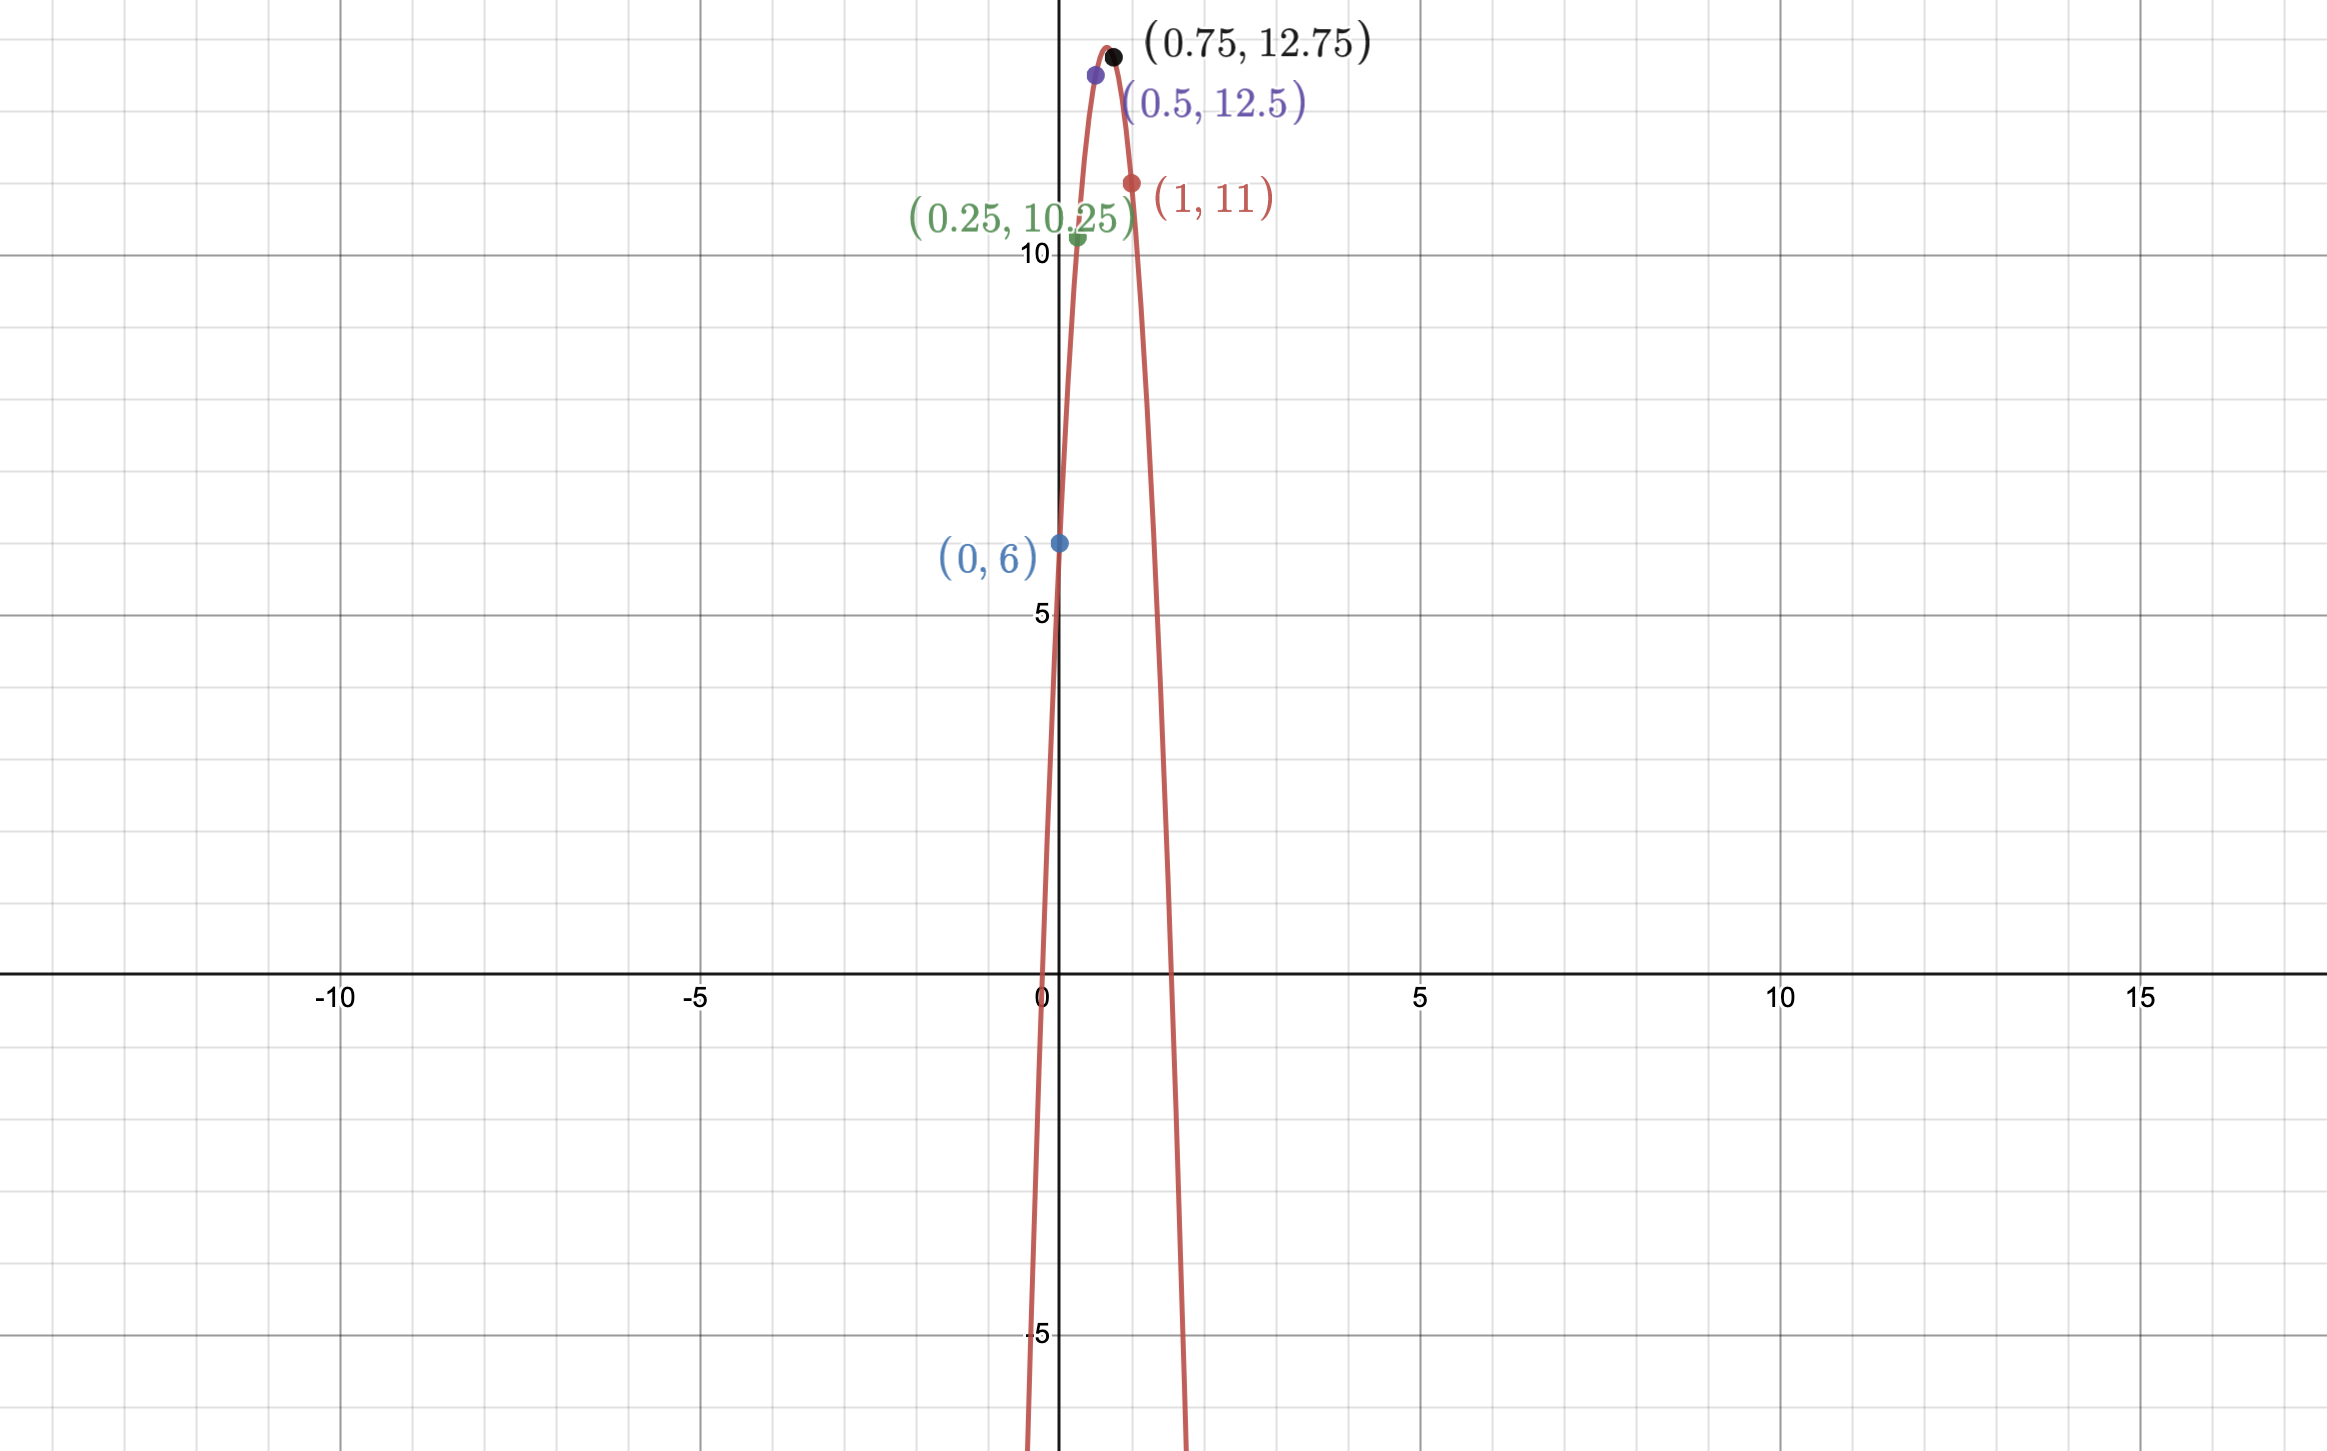
\includegraphics[width = 4in, height = 4in]{1.8screenshot1}
\newline
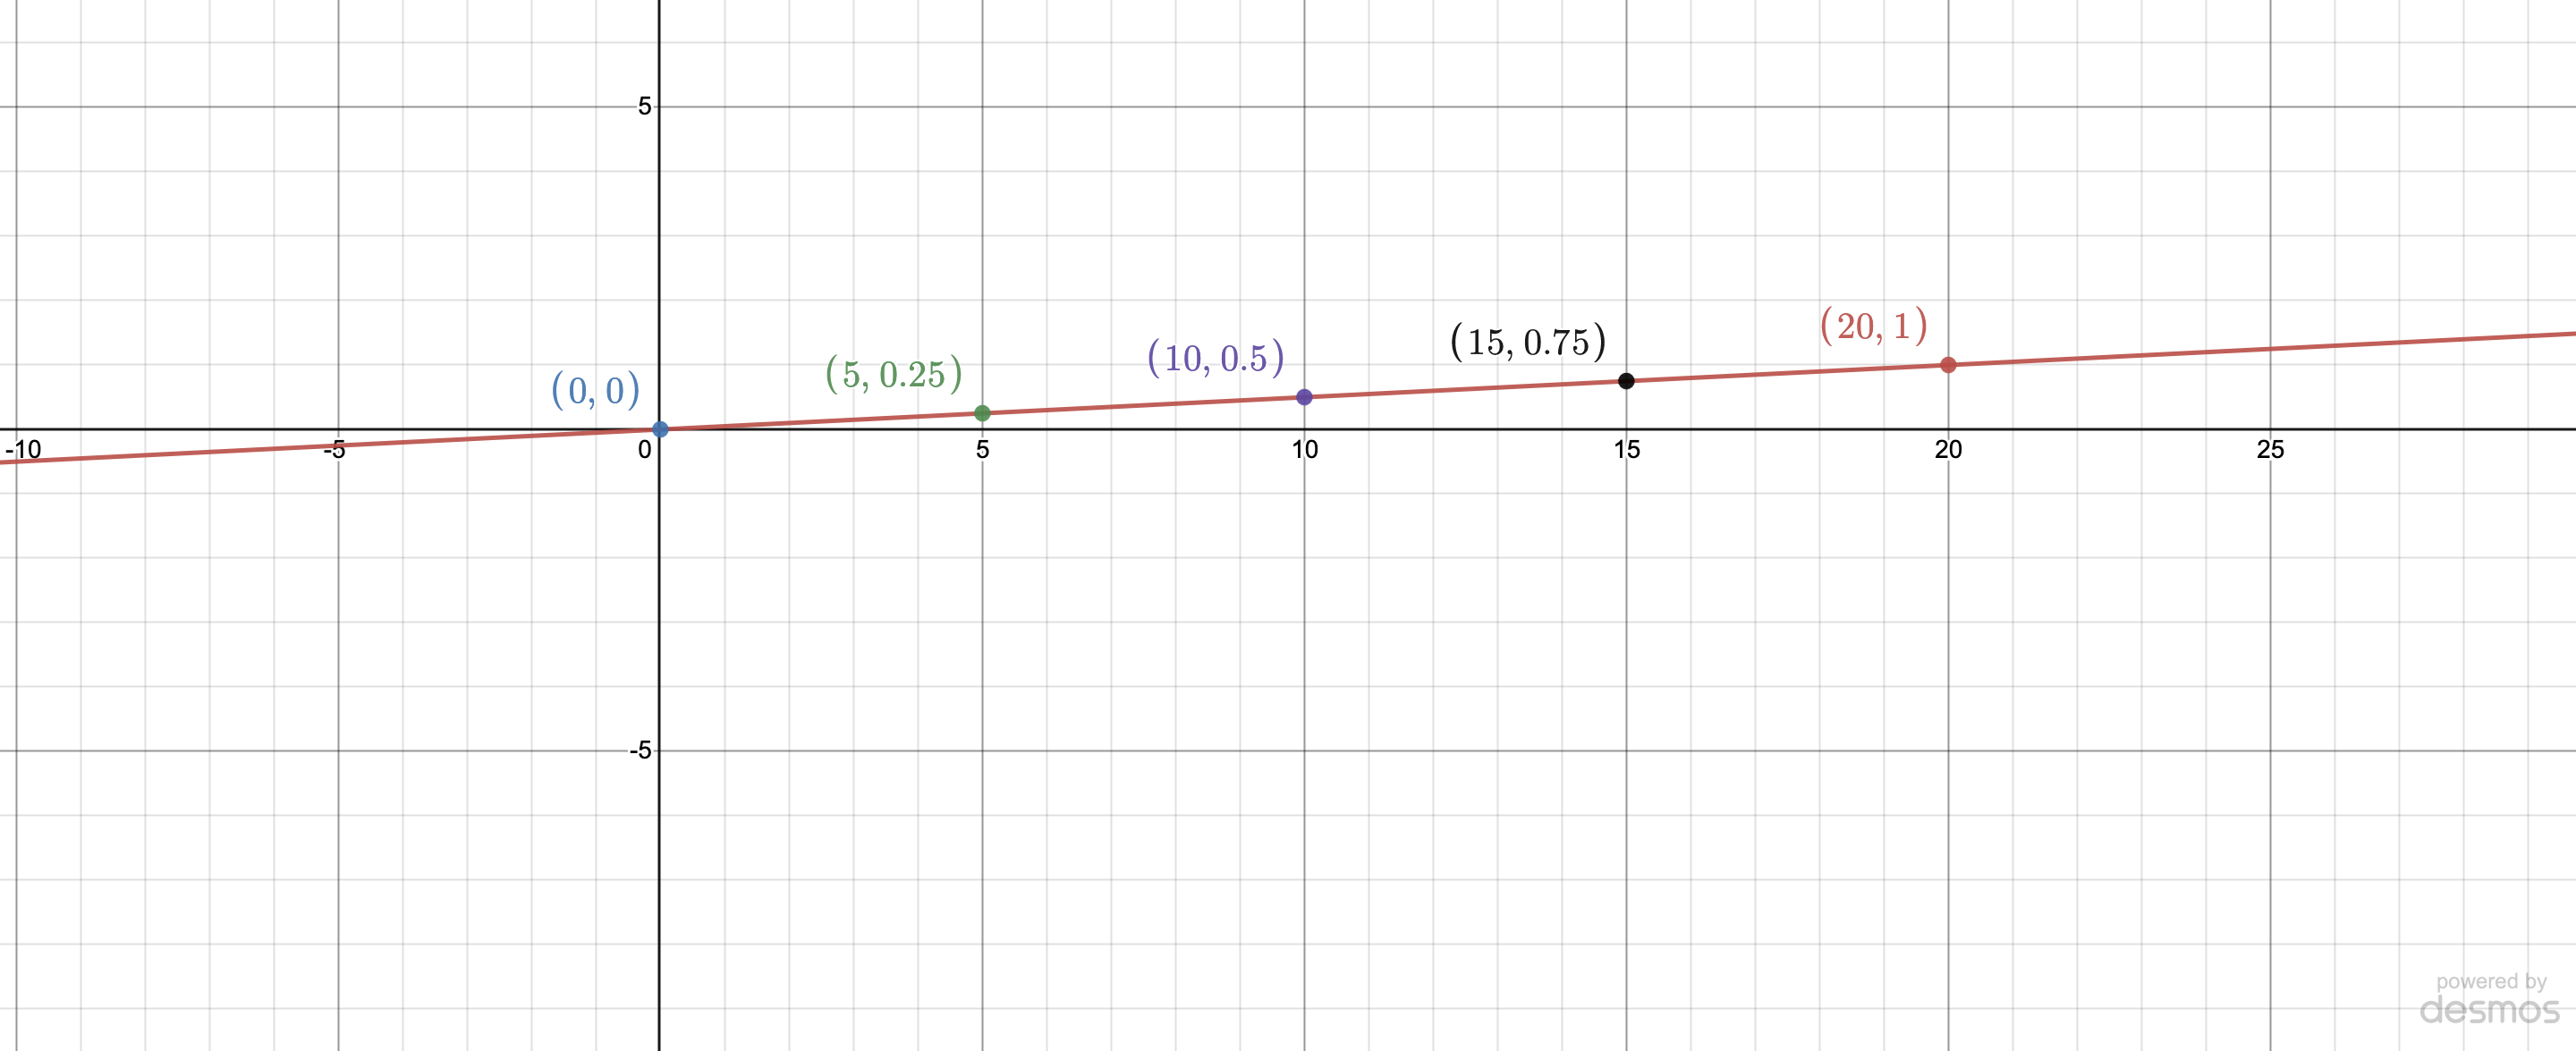
\includegraphics[width = 4in, height = 4in]{1.8screenshot2}\newline
(c) (I was not sure what it meant to make the free throw, but my best guess was that it meant that there was a given time when the basketball 
hits the rim or the backboard):\newline
If the player made the free throw, the ball would hit the basketball rim, or the backboard at a given time. In the first case of the rim, 
we would have $15=20t$ and $10=-16t^2+21t+6$\newline The first equations has $t=0.75$, while the solutions to the second equation are:\newline 
$-16t^2+21t-4=0\newline\rightarrow 
t=\frac{-21\pm\sqrt{21^2-4(-16)(-4)}}{2(-16)}\newline\rightarrow 
t=\frac{-21\pm\sqrt{185}}{-32}\newline\rightarrow 
t=0.231\vee t=1.081$\newline because neither of these values are $0.75$, there is not a value for $t$ such that the ball hits the rim. On the other hand, 
if the ball hit the backboard, we would have $15=20t$ and $12=-16t^2+21t+6$ and again have $t=0.75$ from the first equation, while the solutions to the 
second equation are:\newline 
$-16t^2+21t-6=0\newline\rightarrow 
t=\frac{-21\pm\sqrt{21^2-4(-16)(-6)}}{2(-16)}\newline\rightarrow 
t=\frac{-21\pm\sqrt{57}}{-32}\newline\rightarrow 
t=0.420\vee t=0.892$\newline because neither of these values are $0.75$, there is not a value for $t$ such that the ball hits the backboard, thus meaning 
the palyer does not make the free throw.

\section*{74}
(a): We are given that the maximum value for $h$ is $1081$ ft. The maxmimum value can be found by plugging in the $x$-coordinate of the vertex in 
for $t$, and the $x$-coordinate of the vertex can be found form $-\frac{v_0}{2(-16)}$. Hence, we can plug this value in for $t$ in the equation when 
$h=1081$ and be able to solve for $v_0$:\newline 
$1081=-16(-\frac{v_0}{-32})^2-\frac{v_0}{-32}v_0+921\newline\rightarrow 
160=-\frac{1}{64}v_0^2+\frac{1}{32}v_0^2\newline\rightarrow 
160=\frac{1}{64}v_0^2
v_0^2=10240\newline\rightarrow 
v_0=\pm 101.193$\newline because the initial vertical velocity must be positive (because the ride is going up), $v_0=101.193$ feet per second.\newline
(b): To find how long it takes to get up the ride using the model $h=-16t^2+101.193t+921$, we need to find the $x$-coordinate of the vertex of this 
equation (the value of $t$ for the maximum value). This is given by $-\frac{101.193}{2(-16)}=3.162$ meaning it takes about $3.162$ seconds for the 
ride to reach the top. When comparing this value to the brochures value of $2$ seconds, there is obviously a large difference of over one second. This is 
probably partly due to rounding (I rounded to three decimal places), and possibly due to slight errors in the model, or a simplification of the time 
given in the brochure.



 



\end{document}
